\documentclass{article}
\usepackage{amsmath, sfmath, multicol, tkz-euclide, array, enumerate, tcolorbox, tabularray, tipa}
\renewcommand{\familydefault}{\sfdefault}
\setlength{\parindent}{0cm}
\pagestyle{empty}
\usepackage[left=1in, top=0.5in, right=1in, bottom=0.5in]{geometry}
\tikzset{>=stealth, label style/.append style={font=\footnotesize}}
\tcbset{colback=white}

\newcounter{example}[section]
\newenvironment{example}[1][]{\refstepcounter{example}\par\medskip
   {\color{red}\textbf{Example~\theexample. #1}}}{\medskip}

\newcommand{\arc}[1]{%
    \setbox9=\hbox{#1}%
    \ooalign{\resizebox{\wd9}{\height}{\texttoptiebar{\phantom{A}}}\cr#1}}

\begin{document}

\section*{Inscribed Angles}

\begin{tcolorbox}[colframe=orange!70!white, coltitle=black, title=\textbf{Today I Can}]
\begin{enumerate}
    \item Find the measure of an inscribed angle.
    \item Find the measure of an angle formed by a tangent and a chord.
\end{enumerate}
\end{tcolorbox}
\smallskip 

\begin{tcolorbox}[colframe=black!20!white, opacitybacktitle=0.1, coltitle=black, title=\textbf{Inscribed Angle}]
An angle whose vertex is on the circle. \newline

\begin{minipage}{0.5\textwidth}
\begin{itemize}
    \item $m\angle A = \frac{1}{2} m \arc{\textit{BC}}$
\end{itemize}
\end{minipage}
\begin{minipage}{0.3\textwidth}
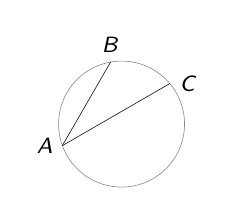
\begin{tikzpicture}[scale=0.8]
\tkzDefPoints{0/0/O}
\tkzDefShiftPoint[O](200:1){A}
\tkzDefShiftPoint[O](100:1){B}
\tkzDefShiftPoint[O](40:1){C}
\tkzDrawCircle(O,A)
\tkzLabelPoints[left](A)
\tkzLabelPoints[above](B)
\tkzLabelPoints[right](C)
\tkzDrawSegments(A,B A,C)
\end{tikzpicture}
\end{minipage}
\end{tcolorbox}
\smallskip 

\begin{example}
Find each measure. \newline 

\begin{minipage}{0.4\textwidth}
    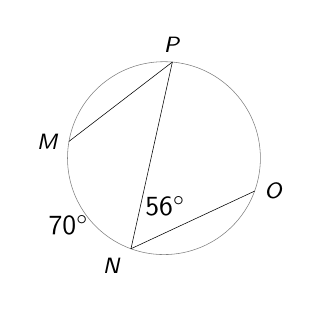
\begin{tikzpicture}[scale=0.7]
    \tkzDefPoints{0/0/A}
    \tkzDefShiftPoint[A](85:1.75){P}
    \tkzDefShiftPoint[A](170:1.75){M}
    \tkzDefShiftPoint[A](250:1.75){N}
    \tkzDefShiftPoint[A](340:1.75){O}
    \tkzDrawCircle(A,P)
    \tkzDrawSegments(M,P P,N N,O)
    \tkzLabelPoints[above](P)
    \tkzLabelPoints[left](M)
    \tkzLabelPoints[below left](N)
    \tkzLabelPoints[right](O)
    \tkzLabelAngle[pos=3.5](M,P,N){$70^\circ$}
    \tkzLabelAngle(O,N,P){$56^\circ$}
    \end{tikzpicture}
\end{minipage}
\begin{minipage}{0.3\textwidth}
\begin{multicols}{2}
\begin{enumerate}[(a)]
    \item $m\angle P$
    \item $m \arc{\textit{PO}}$
\end{enumerate}
\end{multicols}
\end{minipage}
\end{example}

\begin{tcolorbox}[colframe=black!20!white, opacitybacktitle=0.1, coltitle=black, title=\textbf{Congruent Inscribed Angles Theorem}]
If two inscribed angles of a circle intercept the same arc or congruent arcs, then the angles are congruent. \newline

\begin{minipage}{0.5\textwidth}
\begin{itemize}
    \item $\angle A \cong \angle D$
\end{itemize}
\end{minipage}
\begin{minipage}{0.3\textwidth}
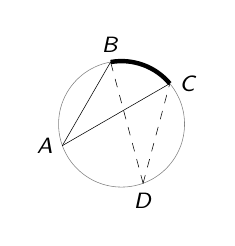
\begin{tikzpicture}[scale=0.8]
\tkzDefPoints{0/0/O}
\tkzDefShiftPoint[O](200:1){A}
\tkzDefShiftPoint[O](100:1){B}
\tkzDefShiftPoint[O](40:1){C}
\tkzDefShiftPoint[O](290:1){D}
\tkzDrawCircle(O,A)
\tkzLabelPoints[left](A)
\tkzLabelPoints[above](B)
\tkzLabelPoints[right](C)
\tkzLabelPoints[below](D)
\tkzDrawSegments(A,B A,C)
\tkzDrawSegments[dashed](D,B D,C)
\draw[ultra thick] (40:1) arc (40:100:1);
\end{tikzpicture}
\end{minipage}
\end{tcolorbox}
\smallskip 

\begin{example}
 Find each given the circle below.
\begin{multicols}{2}
\begin{enumerate}[(a)]
    \item Find $m\angle T$ if $m\angle T = 3x-5$ and $m\angle U=2x+15$.
    \item Find $x$ if $m\angle S=3x$ and $m\angle V=x+16$.
\end{enumerate}
\end{multicols}
\begin{minipage}{0.5\textwidth}
    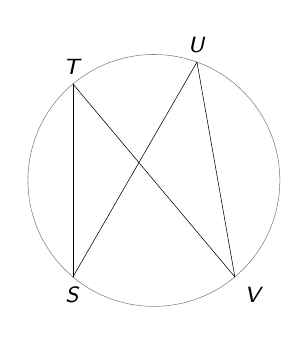
\begin{tikzpicture}[scale=0.8]
    \tkzDefPoints{0/0/A}
    \tkzDefShiftPoint[A](70:2){U}
    \tkzDefShiftPoint[A](130:2){T}
    \tkzDefShiftPoint[A](230:2){S}
    \tkzDefShiftPoint[A](310:2){V}
    \tkzDrawCircle(A,U)
    \tkzDrawSegments(S,T T,V V,U U,S)
    \tkzLabelPoints[above](T,U)
    \tkzLabelPoints[below](S)
    \tkzLabelPoints[below right](V)
    \end{tikzpicture}
\end{minipage}
\begin{minipage}{0.4\textwidth}
    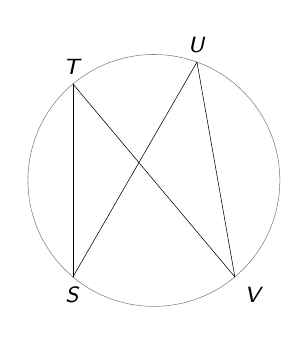
\begin{tikzpicture}[scale=0.8]
    \tkzDefPoints{0/0/A}
    \tkzDefShiftPoint[A](70:2){U}
    \tkzDefShiftPoint[A](130:2){T}
    \tkzDefShiftPoint[A](230:2){S}
    \tkzDefShiftPoint[A](310:2){V}
    \tkzDrawCircle(A,U)
    \tkzDrawSegments(S,T T,V V,U U,S)
    \tkzLabelPoints[above](T,U)
    \tkzLabelPoints[below](S)
    \tkzLabelPoints[below right](V)
    \end{tikzpicture}
\end{minipage}
\end{example}

\begin{tcolorbox}[colframe=black!20!white, opacitybacktitle=0.1, coltitle=black, title=\textbf{Thales Theorem}]
An angle inscribed in a semi-circle is a right angle. \newline

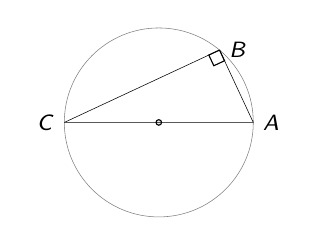
\begin{tikzpicture}[scale=0.6]
    \tkzDefPoints{0/0/O, 2/0/A, -2/0/C}
    \tkzDefShiftPoint[O](50:2){B}
    \tkzDrawCircle(O,A)
    \tkzDrawPoint(O)
    \tkzDrawPolygon(O,A,B,C)
    \tkzMarkRightAngle(A,B,C)
    \tkzLabelPoints[right](A,B)
    \tkzLabelPoints[left](C)
\end{tikzpicture}
\end{tcolorbox}
\smallskip 

\begin{example}
Find $x$ in each given the circle below.
\begin{multicols}{2}
\begin{enumerate}[(a)]
    \item $m\angle F = 4x+2$ and $m\angle H=9x-3$.
    \item $m\angle F = 7x+2$ and $m\angle H=17x-8$.
\end{enumerate}
\end{multicols}
\begin{minipage}{0.5\textwidth}
    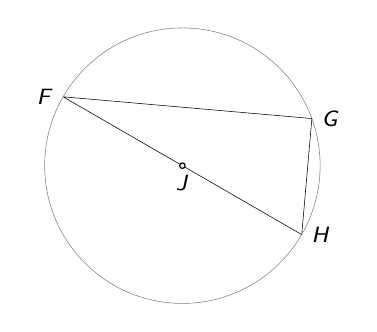
\begin{tikzpicture}[scale=0.7]
    \tkzDefPoints{0/0/J}
    \tkzDefShiftPoint[J](20:2.5){G}
    \tkzDefShiftPoint[J](150:2.5){F}
    \tkzDefShiftPoint[J](330:2.5){H}
    \tkzDrawPolygon(F,G,H)
    \tkzDrawCircle(J,G)
    \tkzDrawPoint(J)
    \tkzLabelPoints[below](J)
    \tkzLabelPoints[left](F)
    \tkzLabelPoints[right](G,H)
    \end{tikzpicture}
\end{minipage}
\begin{minipage}{0.4\textwidth}
    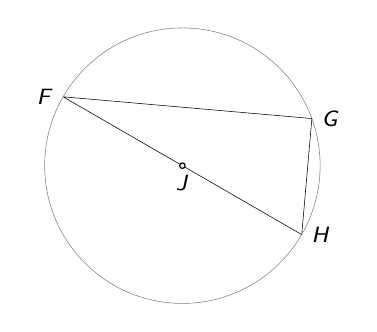
\begin{tikzpicture}[scale=0.7]
    \tkzDefPoints{0/0/J}
    \tkzDefShiftPoint[J](20:2.5){G}
    \tkzDefShiftPoint[J](150:2.5){F}
    \tkzDefShiftPoint[J](330:2.5){H}
    \tkzDrawPolygon(F,G,H)
    \tkzDrawCircle(J,G)
    \tkzDrawPoint(J)
    \tkzLabelPoints[below](J)
    \tkzLabelPoints[left](F)
    \tkzLabelPoints[right](G,H)
    \end{tikzpicture}
\end{minipage}
\end{example}

\vfill 

\begin{tcolorbox}[colframe=black!20!white, opacitybacktitle=0.1, coltitle=black, title=\textbf{Quadrilateral Inscribed in a Circle}]
If a quadrilateral is inscribed in a circle then its opposite angles are supplementary. \newline

\begin{minipage}{0.5\textwidth}
\begin{itemize}
    \item $\angle A$ and $\angle C$ are supplementary.
    \item $\angle B$ and $\angle D$ are supplementary.
\end{itemize}
\end{minipage}
\begin{minipage}{0.4\textwidth}
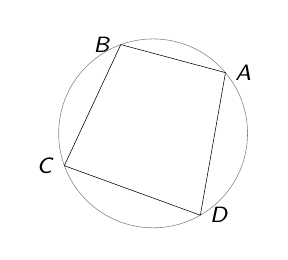
\begin{tikzpicture}[scale=0.6]
    \tkzDefPoints{0/0/O}
    \tkzDefShiftPoint[O](40:2){A}
    \tkzDefShiftPoint[O](110:2){B}
    \tkzDefShiftPoint[O](200:2){C}
    \tkzDefShiftPoint[O](300:2){D}
    \tkzDrawCircle(O,A)
    \tkzDrawPolygon(A,B,C,D)
    \tkzLabelPoints[right](A,D)
    \tkzLabelPoints[left](B,C)
\end{tikzpicture}
\end{minipage}
\end{tcolorbox}
\smallskip

\begin{example}
Find the $m\angle A$ and $m\angle B$.
\newline

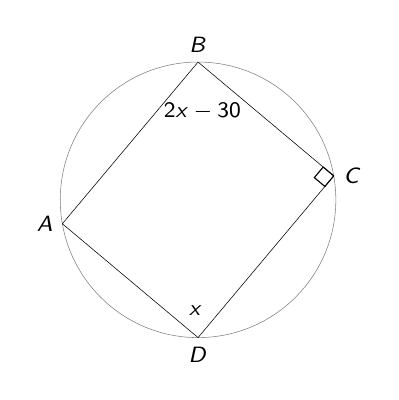
\begin{tikzpicture}[scale=0.7]
\tkzDefPoints{0/0/O, 0/-2.5/D, 0/2.5/B}
\tkzDrawCircle(O,D)
\tkzDefShiftPoint[O](10:2.5){C}
\tkzDefShiftPoint[O](190:2.5){A}
\tkzDrawPolygon(A,B,C,D)
\tkzLabelPoints[left](A)
\tkzLabelPoints[below](D)
\tkzLabelPoints[right](C)
\tkzLabelPoints[above](B)
\tkzMarkRightAngle(D,C,B)
\tkzLabelAngle[pos=0.5](C,D,A){\footnotesize $x$}
\tkzLabelAngle[pos=0.9](A,B,C){\footnotesize $2x-30$}
\end{tikzpicture}
\end{example}

\vfill 

\end{document}
